\documentclass[12pt, letterpaper]{report}   % Single-sided printing for the library

% TOGGLE ON TO SEE PAGE MARGINS -- useful to check that your figures and tables don't go over the specified margins - HG 2018
% \usepackage[showframe]{geometry}

\usepackage[bf]{caption} % Make nice captions with bold "Figure..." and "Table..."
\setcaptionmargin{0.5in}
%package for the bu thesis format -- most commonly-used packages added in the style file by HG 2018
\usepackage{bu_math_thesis}

\graphicspath{{figures/}{tables/}}

%%%%%%%%%%%%%%%%%%%%%%%%%%%%%%%%%%%%%%%%%%%%%%%%%%%%%%%%%%%%%%%%%%%%%%%%%%
%define the frequent formulas shorthands for typing -- note that these do not appear as the function in "Rich Text" format in Overleaf, but rather as the "\shorthand"

\newcommand{\lagin}{\ensuremath{\lambda_{1}}}
\newcommand{\lagout}{\ensuremath{\lambda_{2}}}

%%%%%%%%%%%%%%%%%%%%%%%%%%%%%%%%%%%%%%%%%%%%%%%%%%%%%%%%%%%%%%%%%%%%%%%%%%
\begin{document}
%%%%%%%%%%%%%%%%%%%%%%%%%%%%%%%%%%%%%%%%%%%%%%%%%%%%%%%%%%%%%%%%%%%%%%%%%%
% Setup commands for the bu thesis style file

\title{This is the final title for my dissertation}
\author{Joe Candidate}

% Type of document prepared for this degree:
%   2 = Doctor of Philosophy dissertation.
%   4 = Doctoral Dissertation Prospectus
\degree=2

% List your bachelors degree before your masters - HG 2018
\prevdegrees{BA in Mathematics, Undergrad College, 2008\\
MA in Biostatistics, Boston University, 2012}
\department{Department of Biostatistics}
\university{Boston University}
\faculty{Graduate School of Arts and Sciences}

% Degree year is the year the diploma is expected, and defense year is the year the dissertation is written up and defended. Often, these will be the same, except for January graduation, when your defense will be in the fall of year X, and your graduation will be in January of year X+1
\defenseyear{2018}
\degreeyear{2018}

% For each reader, specify appropriate label {First, second, third}, then name, then title. Warning: If you have more than five readers you are out of luck, because it will overflow to a new page. Sometimes you may wish to put part of the title in with the name
% Do NOT put the chair on your approval page - HG 2018
\reader{First}{Primary Advisor, MD MPH PhD}{Research Professor, Biostatistics}
\reader{Second}{Second reader, PhD}{Professor, Biostatistics}
\reader{Third}{Third reader, ScD}{Assistant Professor,  Biostatistics}
\reader{Fourth}{Fourth reader, PhD}{Adjunct Professor,  Biostatistics}

% The Major Professor is the same as the first reader, but must be specified again for the abstract page
% Just copy and paste the same information
\majorprof{Primary Advisor}{MD MPH PhD}


%%%%%%%%%%%%%%%%%%%%%%%%%%%%%%%%%%%%%%%%%%%%%%%%%%%%%%%%%%%%%%%%%%%%%
% other set up commands which are a good idea

%the bottom margins should be "as close as possible" to 1 inch, so allowdisplaybreaks is a good idea for theses with a lot of equations
\allowdisplaybreaks


%%%%%%%%%%%%%%%%%%%%%%%%%%%%%%%%%%%%%%%%%%%%%%%%%%%%%%%%%%%%%%%%%%%%%
%                       PRELIMINARY PAGES
% According to the BU guide the preliminary pages consist of: title, copyright (optional), approval,  acknowledgments (opt.), abstract, preface (opt.), Table of contents, List of tables (if any), List of illustrations (if any). The \tableofcontents, \listoffigures, and \listoftables commands can be used in the appropriate places. For other things like preface, do it manually with something like \newpage\section*{Preface}.

%%%%%%%%%%%%%%%%%%%%%%%%%%%%%%%%%%%%%%%%%%%%%%%%%%%%%%%%%%%%%%%%%%%%
% This is an additional page (do not hand it in at the library) to print boxed-in title, author and degree statement so that they are visible through the opening in BU covers used for reports. This makes a nicely bound copy.

%\buecethesistitleboxpage

%%%%%%%%%%%%%%%%%%%%%%%%%%%%%%%%%%%%%%%%%%%%%%%%%%%%%%%%%%%%%%%%%%%%
%%%% TITLE PAGE
% Make the titlepage based on the above information.  If you need something special and can't use the standard form, you can specify the exact text of the titlepage yourself.  Put it in a titlepage environment and leave blank lines where you want vertical space. The spaces will be adjusted to fill the entire page.
\maketitle

%%%%%%%%%%%%%%%%%%%%%%%%%%%%%%%%%%%%%%%%%%%%%%%%%%%%%%%%%%%%%%%%%%%%
%%%% COPYRIGHT PAGE
% The copyright page is blank except for the notice at the bottom. You must provide your name in capitals.
\copyrightpage

%%%%%%%%%%%%%%%%%%%%%%%%%%%%%%%%%%%%%%%%%%%%%%%%%%%%%%%%%%%%%%%%%%%%
%%%% APPROVAL PAGE
% Now include the approval page based on the readers information
\approvalpage

%%%%%%%%%%%%%%%%%%%%%%%%%%%%%%%%%%%%%%%%%%%%%%%%%%%%%%%%%%%%%%%%%%%%
%%%% DEDICATION
\addcontentsline{toc}{chapter}{Dedication}
\section*{Dedication}
This dissertation is dedicated to....

%%%%%%%%%%%%%%%%%%%%%%%%%%%%%%%%%%%%%%%%%%%%%%%%%%%%%%%%%%%%%%%%%%%%
%%%% ACKNOWLEDGEMENTS
\newpage
\addcontentsline{toc}{chapter}{Acknowledgements}
\section*{Acknowledgments}

The style file is originally based on an MIT sytle file by Stephen Gildea, modified for BU by Paolo Gaudiano.  Modified for CNS by Jonathan Polimeni.  Further modifications by Janusz Konrad, Cameron Morland, and Karen Yeats. The final version you are using was revised by Hanna Gerlovin to align with current (2018) specifications by GRS for dissertation formatting.

This example file takes some comments from a previous example file of unknown authorship.

%%%%%%%%%%%%%%%%%%%%%%%%%%%%%%%%%%%%%%%%%%%%%%%%%%%%%%%%%%%%%%%%%%%%
%%%% ABSTRACT
\newpage
\addcontentsline{toc}{chapter}{Abstract}
% The abstract page environment sets up everything on the page except the text itself.  The title and other header material are put at the top of the page, and the supervisors are listed at the bottom.  A new page is begun both before and after.  Of course, an abstract may be more than one page itself.  If you need more control over the format of the page, you can use the abstract environment, which puts the word "Abstract" at the beginning and single spaces its text.

% 1.5.1 Purpose in writing the abstract

% The abstract should contain a clear and brief statement of the problem, the procedure(s) and/or method(s) followed, the result(s), and the conclusion(s). The purpose of an abstract is to help a reader decide if they want to consult the complete work. 
% As with the title, the abstract is searchable in many databases, including ProQuest Dissertations & Theses Full Text. Include relevant place names, full personal names, and other proper nouns, which can be very useful keywords for scholars locating resources.

% 1.5.2 Written in English and limited in length

% The abstract must be written in English. A dissertation abstract is limited to 350 words or approximately 2,450 characters. A thesis abstract is limited to 250 words or approximately 1,750 characters.

\begin{abstractpage}
The abstract must be written in English. A dissertation abstract is limited to 350 words or approximately 2,450 characters. A thesis abstract is limited to 250 words or approximately 1,750 characters.
\end{abstractpage}


% Now you can include a preface. Again, use something like
% \newpage\section*{Preface} followed by your text

%%%%%%%%%%%%%%%%%%%%%%%%%%%%%%%%%%%%%%%%%%%%%%%%%%%%%%%%%%%%%%%%%%%%
%%%%% CODE FOR CLEANING UP PDF HYPERLINKS - HG 2018
%remove the hyperlink colors for table of contents
\begingroup
  \hypersetup{linkbordercolor=white,linkcolor=black,
    filecolor=black, urlcolor=black}

%%%%%%%%%%%%%%%%%%%%%%%%%%%%%%%%%%%%%%%%%%%%%%%%%%%%%%%%%%%%%%%%%%%%
%%%% TABLE OF CONTENTS
% Table of contents comes after preface
\tableofcontents


%%%%%%%%%%%%%%%%%%%%%%%%%%%%%%%%%%%%%%%%%%%%%%%%%%%%%%%%%%%%%%%%%%%%
%%%% LIST OF TABLES
% If you have tables this goes here - needs to be in appendix HG 2018
\newpage
\addcontentsline{toc}{chapter}{List of Tables}
\listoftables

%%%%%%%%%%%%%%%%%%%%%%%%%%%%%%%%%%%%%%%%%%%%%%%%%%%%%%%%%%%%%%%%%%%%
%%%% LIST OF FIGURES
% If you have figures this goes here - needs to be in appendix HG 2018
\newpage
\addcontentsline{toc}{chapter}{List of Figures}
\listoffigures
\endgroup

%%%%%%%%%%%%%%%%%%%%%%%%%%%%%%%%%%%%%%%%%%%%%%%%%%%%%%%%%%%%%%%%%%%%
%%%% LIST OF SYMBOLS AND ABBREVIATIONS
% List of Abbrevs is NOT optional (PUT IN ALPHABETICAL ORDER)
% For mathematics a list of symbols is perhaps more appropriate, but fulfills the same role
\newpage
\addcontentsline{toc}{chapter}{List of Symbols and Abbreviations}
\chapter*{List of Symbols and Abbreviations}\label{RefSymbols}
  \begin{longtable}{lp{0.75\textwidth}}
    AIC \dotfill & Akaike's Information Criterion \\
    CI \dotfill & Confidence Interval \\
    CP \dotfill & Coverage Probability \\
    HR \dotfill & Hazard Ratio \\
	PLR \dotfill & Pooled Logistic Regression\\
\end{longtable}

% END OF THE PRELIMINARY PAGES
\newpage
\endofprelim
\cleardoublepage

%%%%%%%%%%%%%%%%%%%%%%%%%%%%%%%%%%%%%%%%%%%%%%%%%%%%%%%%%%%%%%%%%%
% the body of the thesis goes here.
\chapter{Introduction}
\label{introduction}

This is an introduction to using the \LaTeX \xspace template for writing your PhD Dissertation.

\section{Equations}

Here is a simple equation that I would like to reference at a later point. I have labeled it \verb+\label{eq:OCM2}+.
\begin{equation} \label{eq:OCM2}
C_{p}^{ss}=\dfrac{k_0}{k_{e}V}
\end{equation}

For equations that just need to be shown, but not referenced, you can use \verb+$$\dfrac{1}{2}$$+ to center the lines
$$\dfrac{1}{2}=1-e^{-k_{e}t_{h}}\longrightarrow\frac{1}{2}=e^{-k_{e}t_{h}}\longrightarrow\ln⁡{(\dfrac{1}{2})}=\ln{(1)}-\ln{(2)}=-\ln{(2)}=-k_{e}t_{h}$$

\section{Some important background}
I have some literature that I would like to cite.\citep{Cole2014,Venzon1988,Murphy2000,Sprott2000} To use the author's name inline, I can refer to \citet{Cox1992} this way. 

\subsection{Footnote citation}
Figure \ref{fig:proflike} (on page \pageref{fig:proflike}) was pulled as a ".png" file from online and I would like to cite it in a footnote.\footnote{Image taken from: https://www.unc.edu/courses/2010fall/ecol/563/001/images/lectures/\\lecture8/fig4new.png}

\section{Margins} \label{ch1:Description}
Here is a small intro into sentences that break the margins. Hint: you can see this by "toggling on" the \verb+\usepackage[showframe]{geometry}+ line in the dissertation.tex file (at the top).

"If I want to reference something that was done in chapter \ref{chapter2}, I can type \verb+\ref{chapter2}+."

Notice that the previous paragraph breaks the page margins! This can happen when you use shorthand or other notations/equations that have trouble identifying the length of a line from the placeholder text. To fix this try putting the paragraph into \verb+\begin{sloppypar}...\end{sloppypar}+ as follows:

\begin{sloppypar}
If I want to reference something that was done in chapter \ref{chapter2}, I can type \verb+\ref{chapter2}+. 
\end{sloppypar}

\cleardoublepage
\chapter{Chapter 2 Title}
\label{sec:chap2}
\thispagestyle{myheadings}

\section{This Section Title}
\label{sec:thissec}

Lorem ipsum dolor sit amet, consectetur adipiscing elit. Praesent nec velit magna. In vehicula accumsan blandit. Duis vestibulum eros et ante posuere et pharetra nibh dapibus. Pellentesque quis nibh vestibulum urna fermentum convallis. Duis ultricies felis eget orci sodales sed varius ante facilisis. Vivamus nec lorem nulla. Donec id quam id arcu fringilla euismod. Etiam ullamcorper posuere ipsum, vel egestas ipsum bibendum faucibus. Proin volutpat dolor vel nulla egestas in ultricies mi pellentesque. Vivamus ut nulla ligula. 

%%###############################################################################################

\subsection{Subsection}
\label{sec:subsec}

Lorem ipsum dolor sit amet, consectetur adipiscing elit. Praesent nec velit magna. In vehicula accumsan blandit. Duis vestibulum eros et ante posuere et pharetra nibh dapibus. Pellentesque quis nibh vestibulum urna fermentum convallis. Duis ultricies felis eget orci sodales sed varius ante facilisis. Vivamus nec lorem nulla. Donec id quam id arcu fringilla euismod. Etiam ullamcorper posuere ipsum, vel egestas ipsum bibendum faucibus. Proin volutpat dolor vel nulla egestas in ultricies mi pellentesque. Vivamus ut nulla ligula. 

\cleardoublepage
\chapter{Final Set of Examples}
\label{chapter3}

\section{Tables and Figures}

\subsection{Inline Table Example}
\begin{table}[h]
	\caption{Example set of tables side-by-side using minipage} 
	\centering
	\begin{minipage}[b]{0.30\linewidth}
		\centerline{$\eta=6000$, $\mu=2000$}\smallskip
		\centering
		\begin{tabular}{ccc}
			\hline
			$K$ & $u_1$ & $u_2$\\
			\hline
			3   & 0.52 &0.46\\
			7   & 0.47 &0.43\\
			12  & 0.37 &0.36\\
			\hline
		\end{tabular}
	\end{minipage}
	\begin{minipage}[b]{0.34\linewidth}
		\centerline{$K=10$, $\mu=2000$}\smallskip
		\centering
		\begin{tabular}{ccc}
			\hline
			$\eta$ & $u_1$ & $u_2$\\
			\hline
			1000&0.54& 0.45\\
			3000&0.43& 0.40\\
			9000&0.37& 0.37\\
			\hline
		\end{tabular}
	\end{minipage}
	\begin{minipage}[b]{0.32\linewidth}
		\centerline{$K=10$, $\eta=6000$}\smallskip
		\centering
		\begin{tabular}{ccc}
			\hline
			$\mu$ & $u_1$ & $u_2$\\
			\hline
			100 &1.00&1.16\\
			1000&0.53&0.47\\
			3000&0.44&0.43\\
			\hline
		\end{tabular}
	\end{minipage}
	\label{tab:threetabs}
\end{table}
\cleardoublepage

%%%%%%%%%%%%%%%%%%%%%%%%%%%%%%%%%%%%%%%%%%%%%%%%%%%%%%%%%%%%%%%%%%
% Quick references for some R packages used that I want in the bibliography
\nocite{tikzDevice,plotly,reshape,Rcomputing,Florida2000}

%%%%%%%%%%%%%%%%%%%%%%%%%%%%%%%%%%%%%%%%%%%%%%%%%%%%%%%%%%%%%%%%%%
% Put your appendices inside here, to maintain figure and table listings. Make sure to use \section{appendixA} to have some numbering for figures and tables.
\begin{appendices}
\chapter*{Glossary of Terms}
\label{glossary}
\begin{longtable}{r p{0.6\textwidth}}
    \textbf{\textit{Complicated Term}}: & Make sure to define anything that you allude to in the text\\
    \textbf{\textit{Parameter}}: & Description of the parameter. This is not the same as the List of Symbols. \\
\end{longtable}
\chapter{Special Stuff}
\label{AppA}

\section{Appendix Tables}
If you plan on using tables and/or figures in an Appendix, make sure that you use \verb+\chapter{}+ instead of \verb+\chapter*{}+. This is to ensure that your figures and tables that are included in the Appendix have a leading letter for enumeration. 

\begin{figure}[H] %"H" says to put the figure in that exact location
\centering
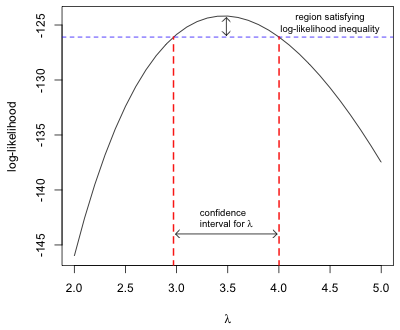
\includegraphics[width=0.7\textwidth]{./figures/proflike_example}
\caption[External figure]{Caption line below the figure.} % Caption line pasted below puts \includegraphics[]{} the caption below the figure. 
\label{fig:proflike}
\end{figure}
\end{appendices}
%%%%%%%%%%%%%%%%%%%%%%%%%%%%%%%%%%%%%%%%%%%%%%%%%%%%%%%%%%%%%%%%%%%%
% The back matter



%%%%%%%%%%%%%%%%%%%%%%%%%%%%%%%%%%%%%%%%%%%%%%%%%%%%%%%%%%%%%%%%%%%%
%%%% LIST OF JOURNAL ABBREVIATIONS
% If you don't write the journal names out in full in the bibliography then you need a list of journal abbreviations
\chapter*{List of Journal Abbreviations}
% I have included a list of common journals that are used in Biostatistics. Make sure that your .bib file abbreviations match what is here. - HG 2018
\begin{center}
\begin{longtable}{lp{0.56\textwidth}}
  Am J Epidemiol \dotfill & American Journal of Epidemiology \\
  Am J Public Health \dotfill & American Journal of Public Health \\
  Am Stat \dotfill & The American Statistician \\
  Ann Intern Med \dotfill & Annals of Internal Medicine \\
  Ann Stat \dotfill & The Annals of Statistics \\
  Arch Intern Med \dotfill & Archives of Internal Medicine \\
  BMJ \dotfill & The British Medical Journal \\
  Can J Stat \dotfill & The Canadian Journal of Statistics \\
  IEEE Trans Automat Contr \dotfill & Institute of Electrical and Electronics Engineers Transactions on Automatic Control \\
  JAMA \dotfill & Journal of the American Medical Association \\
  JASA \dotfill & Journal of the American Statistical Association \\
  J R Stat Soc Ser B \dotfill & Journal of the Royal Statistical Society. Series B (Statistical Methodology) \\
  J R Stat Soc Ser C \dotfill & Journal of the Royal Statistical Society. Series C (Applied Statistics) \\
  J Stat Softw \dotfill & The Journal of Statistical Software \\
  N Engl J Med \dotfill & New England Journal of Medicine \\
  Stat Med \dotfill & Statistics in Medicine 
\end{longtable}
\end{center}


%%%%%%%%%%%%%%%%%%%%%%%%%%%%%%%%%%%%%%%%%%%%%%%%%%%%%%%%%%%%%%%%%%%%
%%%% 	BIBLIOGRAPHY
% The bibliography itself can be single spaced with at least one extra space between items

% 1.8.1 Formatting the bibliography
% Include a complete bibliography at the end of the work. Arrange the bibliography alphabetically by the last name of the primary author. You may single-space citations, but leave one line of space between citations. If you use an article style format, where each chapter has its own separate bibliography, you must also include a cumulative bibliography at the end of the work.
% Verify any other requirements for formatting the bibliography at the end of the work. Certain disciplines/departments may require an alternate arrangement to the bibliography, for example, separating primary and secondary sources and then arranging each alphabetically by last name of author.

\newpage
\singlespace
\Urlmuskip=0mu plus 1mu\relax % Don't let the website links get all funky and break the page margins
\bibliographystyle{apa-good} % technically, you need APA. This style file adds the URL to websites and the date accessed. NOTE: Mendeley API does not put the "date accessed" into the .bib file, so you may want to export directly - HG 2018
\bibliography{Thesis.bib} % keep this on, or you will get warnings about undefined citations


%%%%%%%%%%%%%%%%%%%%%%%%%%%%%%%%%%%%%%%%%%%%%%%%%%%%%%%%%%%%%%%%%%%%
%%%%% CURRICULUM VITAE
% Finally you must include your cv.  You can do that whatever way you like including by formatting it in a totally different program.

% If you would like to grab it from some other source then be sure the page numbering is consecutive with the end of the bibliography and be sure it appears on the table of contents by adding a line such as
% \addcontentsline{toc}{chapter}{Curriculum Vitae}

\chapter*{Curriculum Vitae}
\thispagestyle{empty}
\begin{large}
\begin{center}
\textbf{Your Name, MA}\\
\today\\
\end{center}
\end{large}

\setlength{\columnsep}{1.5in}
\begin{multicols}{2}{
\begin{center}{
Home Street \\ Town, MA 01010 \\ (800) 867 5309 \\ \hyperlink{mailto:personaladdress@gmail.com}{personaladdress@gmail.com}\\
Work office \\Boston University \\ Boston, MA 02118 \\\hyperlink{mailto:buemail@bu.edu}{buemail@bu.edu}\\}
\end{center}}
\end{multicols}

\subsection*{Academic Training:}
\begin{tabular}{p{0.22\textwidth}p{0.7\textwidth}}
05/2018\small(expected) &  PhD Boston University, Boston, MA; Biostatistics\\
05/2012  & MA Boston University, Boston, MA; Biostatistics \\
05/2008  & BA Undergrad College, Undergradville, US; Mathematics \\
\end{tabular}

\subsection*{Doctoral Research:}
\begin{tabular}{p{0.2\textwidth}p{0.72\textwidth}}
\textbf{Title}: & Put your dissertation title \\
\textbf{Thesis advisor}: & Primary Advisor, MD MPH PhD\\
\textbf{Defense date}: & April 4, 2018 \\
\textbf{Summary}: & A few sentences of summary \\
\end{tabular}

\subsection*{Original, Peer Reviewed Publications (newest first):}
% Make sure to be consistent with your CV bibliographic info formatting
\begin{enumerate}
\item Other authors, \underline{Your name}, More Authors. Title of the most recent article published. \emph{Journal where published}. 2018 May 15. doi: 10.1093/xxx. [Epub ahead of print] PubMed ID: \hyperlink{https://www.ncbi.nlm.nih.gov/pubmed/XXX}{XXX}.
\item John Famous and Example Student. \emph{A special case of a well known conjecture}. Fancy Math. J. \textbf{46} no. 3 (2007), 473-490.
\end{enumerate}

\end{document}
